U opent het pati\"entforulier door in het hoofdmenu op de knop ``Pati\"enten''
te klikken.\\
\\
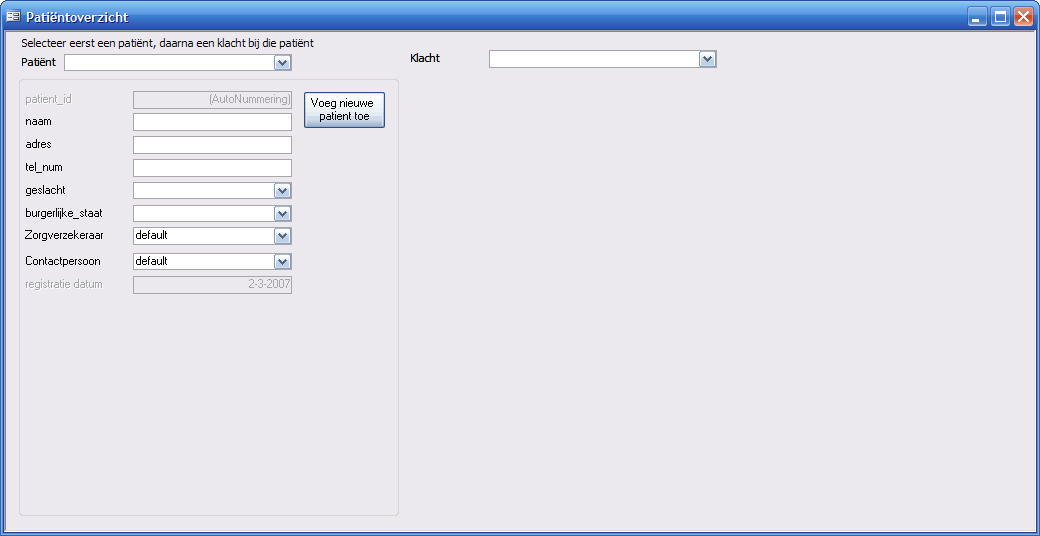
\includegraphics[scale=.5,angle=0]{patient1} \\
\\
In het pati\"entvenster venster kunt U informatie voor en over pati\"enten veranderen,
waaronder geplande opnames, pati\"entinformatie en afspraken. Ook kunt U hier recepten uitschrijven, die bij het apotheekmagazijn kunnen worden opgehaald.

\section{Pati\"entgegevens}
Als er al een pati\"ent bestaat kunt U deze selecteren uit de lijst met pati\"entnamen. Als U een nieuwe pati\"ent wilt toevoegen, klik dan op de knop ``Voeg een nieuwe pati\"ent toe'' en vul vervolgens de informatie over de nieuwe pati\"ent in.

\section{Klachten} \label{sec:klachten}
Om een pati\"ent te kunnen helpen moet de klacht geselecteerd worden uit het rechter uitrol menu. U kunt ook een nieuwe klacht aanmaken door op ``Maak nieuwe klacht aan'' te klikken. Gegevens over de klacht worden in het zonet verschenen venster ingevuld.\\
\\
Nu U de pati\"ent en een klacht heeft geselecteerd kunt U een aantal dingen
doen:
\begin{itemize}
  \item Opnames bekijken, wijzigen en inroosteren.
  \item Recepten uitschrijven, wijzigen en intrekken.
  \item Afspraken bekijken, wijzigen en aanmaken.
  \item De pati\"ent op de wachtlijst zetten voor een operatie.
\end{itemize}

\subsection{Opnames} \label{sec:opnames}
	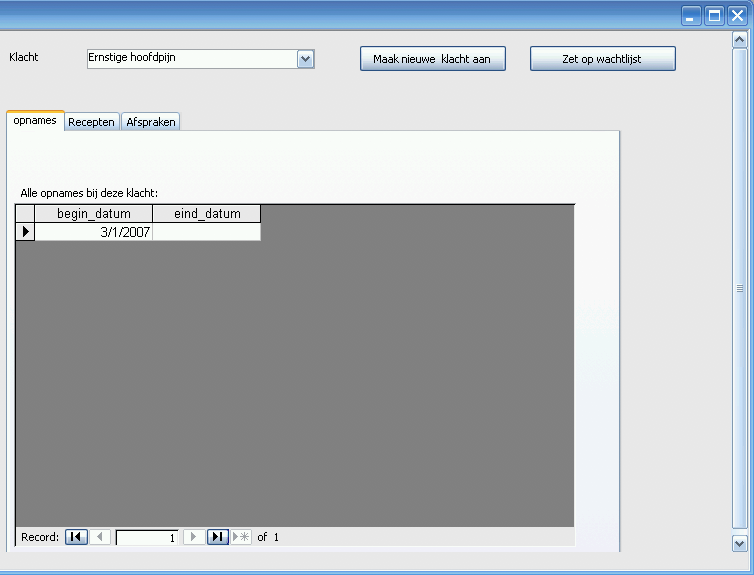
\includegraphics[scale=.5,angle=0]{patient2}\\
  \\
	Het bekijken van opnames doet U door op het tabblad ``Opnames''
        te klikken. Hier staan alle (geplande) begin- en eindtijden van de
	opnames van een pati\"ent. Door op het plusje te klikken voor een
	afspraak, kunt U bekijken (en toevoegen) op welke bedden een pati\"ent
	heeft gelegen tijdens een opname. Elk bed staat op een andere afdeling.

% subsection opnames (end)

\subsection{Recepten} \label{sec:recepten}
	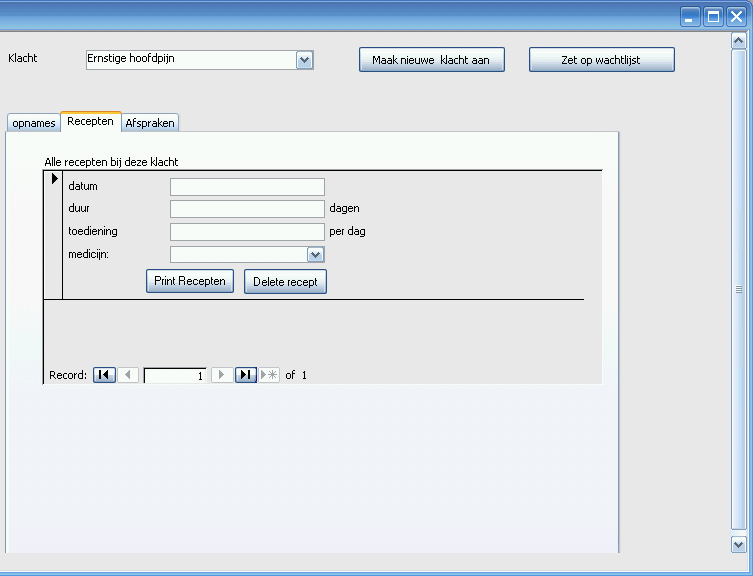
\includegraphics[scale=.5,angle=0]{patient3}\\
  \\
	Het bekijken van recepten doet U door op het tabblad recepten
        te klikken. Hier kunt U recepten bekijken en uitschrijven met de knoppen
	``Print Recepten'' en ``Delete Recept''. Met de pijltjes
	kunt U bladeren door de verschillende recepten bij de geselecteerde klacht.
	
% subsection recepten (end)

\subsection{Afspraken} \label{sec:afspraken}
  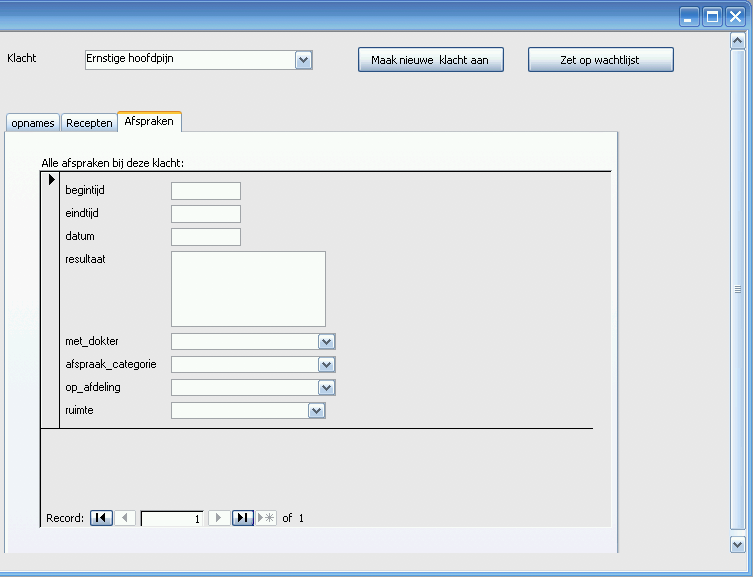
\includegraphics[scale=.5,angle=0]{patient4}\\
  \\
  Het bekijken van afspraken doet U door op het tabblad
	``Afspraken'' te klikken. Hier kunt U de afspraken voor de huidige pati\"ent bekijken	(via de pijltjes onderaan). Ook kunt U een nieuwe afspraak	aanmaken door op het ``nieuwe record'' knopje (met het pijltje sterretje symbool) te klikken.

% subsection afspraken (end)

\subsection{Wachtlijst} \label{sec:wachtlijst}
	U kunt een pati\"ent voor operatie op de wachtlijst zetten met de knop ``Zet
	op wachtlijst'' waarna automatisch de juiste pati\"ent en case wordt geselecteerd,
	zie hiervoor verder de handleiding voor het venster wachtlijst.

% subsection wachtlijst (end)

% section klachten (end) 